% Options for packages loaded elsewhere
\PassOptionsToPackage{unicode}{hyperref}
\PassOptionsToPackage{hyphens}{url}
\PassOptionsToPackage{dvipsnames,svgnames,x11names}{xcolor}
%
\documentclass[
  10pt,
  a4paper,
]{scrreprt}

\usepackage{amsmath,amssymb}
\usepackage{iftex}
\ifPDFTeX
  \usepackage[T1]{fontenc}
  \usepackage[utf8]{inputenc}
  \usepackage{textcomp} % provide euro and other symbols
\else % if luatex or xetex
  \usepackage{unicode-math}
  \defaultfontfeatures{Scale=MatchLowercase}
  \defaultfontfeatures[\rmfamily]{Ligatures=TeX,Scale=1}
\fi
\usepackage{lmodern}
\ifPDFTeX\else  
    % xetex/luatex font selection
\fi
% Use upquote if available, for straight quotes in verbatim environments
\IfFileExists{upquote.sty}{\usepackage{upquote}}{}
\IfFileExists{microtype.sty}{% use microtype if available
  \usepackage[]{microtype}
  \UseMicrotypeSet[protrusion]{basicmath} % disable protrusion for tt fonts
}{}
\usepackage{xcolor}
\usepackage[inner=2cm,outer=2cm,top=2cm,bottom=2cm,headsep=22pt,headheight=11pt,footskip=33pt,ignorehead,ignorefoot,heightrounded]{geometry}
\setlength{\emergencystretch}{3em} % prevent overfull lines
\setcounter{secnumdepth}{1}
% Make \paragraph and \subparagraph free-standing
\ifx\paragraph\undefined\else
  \let\oldparagraph\paragraph
  \renewcommand{\paragraph}[1]{\oldparagraph{#1}\mbox{}}
\fi
\ifx\subparagraph\undefined\else
  \let\oldsubparagraph\subparagraph
  \renewcommand{\subparagraph}[1]{\oldsubparagraph{#1}\mbox{}}
\fi


\providecommand{\tightlist}{%
  \setlength{\itemsep}{0pt}\setlength{\parskip}{0pt}}\usepackage{longtable,booktabs,array}
\usepackage{calc} % for calculating minipage widths
% Correct order of tables after \paragraph or \subparagraph
\usepackage{etoolbox}
\makeatletter
\patchcmd\longtable{\par}{\if@noskipsec\mbox{}\fi\par}{}{}
\makeatother
% Allow footnotes in longtable head/foot
\IfFileExists{footnotehyper.sty}{\usepackage{footnotehyper}}{\usepackage{footnote}}
\makesavenoteenv{longtable}
\usepackage{graphicx}
\makeatletter
\def\maxwidth{\ifdim\Gin@nat@width>\linewidth\linewidth\else\Gin@nat@width\fi}
\def\maxheight{\ifdim\Gin@nat@height>\textheight\textheight\else\Gin@nat@height\fi}
\makeatother
% Scale images if necessary, so that they will not overflow the page
% margins by default, and it is still possible to overwrite the defaults
% using explicit options in \includegraphics[width, height, ...]{}
\setkeys{Gin}{width=\maxwidth,height=\maxheight,keepaspectratio}
% Set default figure placement to htbp
\makeatletter
\def\fps@figure{htbp}
\makeatother
\newlength{\cslhangindent}
\setlength{\cslhangindent}{1.5em}
\newlength{\csllabelwidth}
\setlength{\csllabelwidth}{3em}
\newlength{\cslentryspacingunit} % times entry-spacing
\setlength{\cslentryspacingunit}{\parskip}
\newenvironment{CSLReferences}[2] % #1 hanging-ident, #2 entry spacing
 {% don't indent paragraphs
  \setlength{\parindent}{0pt}
  % turn on hanging indent if param 1 is 1
  \ifodd #1
  \let\oldpar\par
  \def\par{\hangindent=\cslhangindent\oldpar}
  \fi
  % set entry spacing
  \setlength{\parskip}{#2\cslentryspacingunit}
 }%
 {}
\usepackage{calc}
\newcommand{\CSLBlock}[1]{#1\hfill\break}
\newcommand{\CSLLeftMargin}[1]{\parbox[t]{\csllabelwidth}{#1}}
\newcommand{\CSLRightInline}[1]{\parbox[t]{\linewidth - \csllabelwidth}{#1}\break}
\newcommand{\CSLIndent}[1]{\hspace{\cslhangindent}#1}

\addtokomafont{disposition}{\rmfamily}
\usepackage{ragged2e}
\usepackage{blindtext}
\makeatletter
\makeatother
\makeatletter
\makeatother
\makeatletter
\@ifpackageloaded{caption}{}{\usepackage{caption}}
\AtBeginDocument{%
\ifdefined\contentsname
  \renewcommand*\contentsname{Table of contents}
\else
  \newcommand\contentsname{Table of contents}
\fi
\ifdefined\listfigurename
  \renewcommand*\listfigurename{List of Figures}
\else
  \newcommand\listfigurename{List of Figures}
\fi
\ifdefined\listtablename
  \renewcommand*\listtablename{List of Tables}
\else
  \newcommand\listtablename{List of Tables}
\fi
\ifdefined\figurename
  \renewcommand*\figurename{Figure}
\else
  \newcommand\figurename{Figure}
\fi
\ifdefined\tablename
  \renewcommand*\tablename{Table}
\else
  \newcommand\tablename{Table}
\fi
}
\@ifpackageloaded{float}{}{\usepackage{float}}
\floatstyle{ruled}
\@ifundefined{c@chapter}{\newfloat{codelisting}{h}{lop}}{\newfloat{codelisting}{h}{lop}[chapter]}
\floatname{codelisting}{Listing}
\newcommand*\listoflistings{\listof{codelisting}{List of Listings}}
\usepackage{amsthm}
\theoremstyle{definition}
\newtheorem{definition}{Definition}[section]
\theoremstyle{remark}
\AtBeginDocument{\renewcommand*{\proofname}{Proof}}
\newtheorem*{remark}{Remark}
\newtheorem*{solution}{Solution}
\makeatother
\makeatletter
\@ifpackageloaded{caption}{}{\usepackage{caption}}
\@ifpackageloaded{subcaption}{}{\usepackage{subcaption}}
\makeatother
\makeatletter
\@ifpackageloaded{tcolorbox}{}{\usepackage[skins,breakable]{tcolorbox}}
\makeatother
\makeatletter
\@ifundefined{shadecolor}{\definecolor{shadecolor}{rgb}{.97, .97, .97}}
\makeatother
\makeatletter
\makeatother
\makeatletter
\makeatother
\ifLuaTeX
  \usepackage{selnolig}  % disable illegal ligatures
\fi
\IfFileExists{bookmark.sty}{\usepackage{bookmark}}{\usepackage{hyperref}}
\IfFileExists{xurl.sty}{\usepackage{xurl}}{} % add URL line breaks if available
\urlstyle{same} % disable monospaced font for URLs
\hypersetup{
  pdftitle={Annual Progress Review},
  pdfauthor={Thomas William Boughen},
  colorlinks=true,
  linkcolor={blue},
  filecolor={Maroon},
  citecolor={Blue},
  urlcolor={Blue},
  pdfcreator={LaTeX via pandoc}}

\title{Annual Progress Review}
\author{Thomas William Boughen}
\date{}

\begin{document}
\cleardoublepage
\thispagestyle{empty}
{\centering
\hbox{}\vskip 0cm plus 1fill
{\Huge\bfseries Annual Progress Review \par}
\vspace{12ex}
{\Large\bfseries Thomas William Boughen \par}
\vspace{3ex}
\vskip 0cm plus 2fill
%{\bfseries\large Doctor of Philosophy \par}
\vspace{3ex}
{\bfseries\large  \par}
\vspace{12ex}
{
\includegraphics[width=0.1\linewidth]{"imgs/University_of_Newcastle_Coat_of_Arms.png"}\par}
%
%
{\bfseries\large Newcastle University \par}
\vspace{3ex}
%
{\bfseries\large School of Mathematics, Statistics and Physics \par}
%
\vspace{12ex}
%{\small Submitted in total fulfilment of the requirements
%of the degree of Doctor of Philosophy \par}
%}
\justifying
\noindent\ifdefined\Shaded\renewenvironment{Shaded}{\begin{tcolorbox}[boxrule=0pt, breakable, frame hidden, borderline west={3pt}{0pt}{shadecolor}, enhanced, sharp corners, interior hidden]}{\end{tcolorbox}}\fi

\hypertarget{extreme-value-theory}{%
\chapter{Extreme Value Theory}\label{extreme-value-theory}}

Extreme value theory is a field focused on studying properties at the
tail ends of distributions where real world data may be scarce and hard
to make inferences from. A lot of the standard theory assumes continuous
distributions and that is what will be introduced first before looking
at what has been done relating to discrete distributions.

\hypertarget{standard-theory}{%
\section{Standard Theory}\label{standard-theory}}

One approach for modelling the extreme values is to look at modelling
the block maxima of independent and identically distributed random
variables \(X_1,X_2 \ldots\) that all have a common cumulative
distribution function (CDF) \(F\). The block maxima \(M_n\) being
defined as \(M_n = \max\{X_1,\ldots,X_n\}\) has its own CDF defined by:

\[
\Pr(M_n\le x) = F_n(x)
\]

\(F\) is in the domain of attraction of an extreme value CDF \(G\), if
and only if the normalised version of \(M_n\)'s CDF converges to a non
degenerate \(G\), that is, there exists some sequence of \(a_n>0\) and
\(b_n \in \mathbb R\) such that:

\[
\Pr\left(\frac{M_n-b_n}{a_n}\le x\right) = F^n(a_nx+b_n) \rightarrow G(x),\qquad \text{as }n\rightarrow\infty
\]

If this holds, then \(F\) is in the domain of attraction of \(G\) which
we will write as \(F\in\mathcal D(G)\). The extreme value theorem states
that is limit CDF \(G\) can be catagorised into one of three types:

\begin{itemize}
\item
  Gumbel: \(\Lambda(x) = \exp\{-\exp(-x)\},\quad x\in \mathbb R\)
\item
  Fréchet: \(\Phi_a(x) = \exp\{-x^{-\alpha}\},\quad x\ge 0,\alpha>0\)
\item
  Weibull: \(\Psi_\alpha(x) = \exp\{-x^{-a}\},\quad x<0,\alpha>0\)
\end{itemize}

\begin{definition}[Generalised Extreme Value
Distribution]\protect\hypertarget{def-gev}{}\label{def-gev}

These three types of distribution can be combined into one single
distribution called the Generalised Extreme Value (\textbf{GEV})
Distribution which has CDF:

\[
G(x) = \exp\left\{-\left(1+\frac{\xi(x-\mu)}{\sigma}\right)^{-1/\xi}\right\}
\]

denoted \(\text{GEV}(\mu, \sigma, \xi)\) for some
\(\mu\in\mathbb R,\sigma>0, \xi \in \mathbb R\) and has support on
\(\{x\in \mathbb R:1+\xi(x-\mu)/\sigma > 0\}\) with each of the three
types being obtained from changing the values of each of the parameters
with \(\xi=0\) taken as the limit:

\begin{itemize}
\item
  Gumbel: \(\text{GEV}(\mu, \sigma,0)\)
\item
  Fréchet: \(\text{GEV}(1, 1,1/\alpha)\)
\item
  Weibull: \(\text{GEV}(-1, -1,-1/\alpha)\)
\end{itemize}

The most important parameter here is \(\xi\) which will be referred to
as the shape parameter as it controls the tail behaviour of the
distribution allowing it to occupy the three domains of attraction.

\end{definition}

\begin{definition}[Heavy
Tails]\protect\hypertarget{def-heavy}{}\label{def-heavy}

There are a few definitions that can be used to define a distribution
that has heavy tails, one that will not be used here is that the tails
of the distribution function are heavier than an exponential. Here, a
distribution with CDF \(F\) will be said to have heavy tails if it is in
the Fréchet domain of attraction with tail index \(\alpha\), or it is in
the Gumbel domain of attraction.

\end{definition}

\begin{definition}[Generalised Pareto
Distribution]\protect\hypertarget{def-gp}{}\label{def-gp}

A related distribution called the Generalised Pareto (\textbf{GP})
Distribution is also often used to model the probability distribution of
threshold excesses, it has the CDF: \[
H(x) = 1-\left(1+\frac{\xi x}{\sigma}\right)^{-1/\xi}
\] denoted \(\text{GP}(\sigma,\xi)\) for some
\(\sigma>0, \xi\in \mathbb R\) it has support on either \((0,\infty)\)
when \(\xi \ge 0\) or \((0,-\sigma/\xi)\) when \(\xi<0\).

\end{definition}

This distribution of often used to model the conditional probability of
iid random variables exceeding some cut-off \(u\). However, like most of
the theory above, it requires iid discrete random variable; in the case
of networks and modelling the degrees of their vertices the focus is on
discrete data so tools to aid in modelling discrete data are required.

\hypertarget{discrete-extremes}{%
\section{Discrete Extremes}\label{discrete-extremes}}

Since the focus of this report is discrete data, theory on discrete
extremes will need to be examined starting with a discrete alternative
to the GP distribution.

\begin{definition}[Integrated Generalised Pareto
Distribution]\protect\hypertarget{def-igp}{}\label{def-igp}

Roughly following Rohrbeck et al. (2018), the integrated generalised
pareto (\textbf{IGP}) distribution can be defined by considering
modelling the random variable \(Y = \lceil X\rceil\) for some continuous
random variable \(X\) with support on the positive real line such that
\(X|X>u \sim \text{GPD}(\sigma_0+\xi u, \xi)\) for
\(\xi\in\mathbb R,u\in\mathbb R^+\). The probability mass function (PMF)
of the IGP distribution can then be defined as:

For values \(y = \lfloor u \rfloor, \lfloor u \rfloor+1, \ldots\) and
\(\xi \in \mathbb R\) and \(u,\sigma_0 \in\mathbb R^+\):

\begin{align*}
\Pr(Y=y | Y>u) &= \Pr(X<y|X>\lfloor u\rfloor) - \Pr(X<y-1|X>\lfloor u\rfloor) \\
&=\left(1+\frac{\xi(y-1-\lfloor u\rfloor)}{\sigma_0 + \xi \lfloor u \rfloor}\right)_+^{-1/\xi} - \left(1+\frac{\xi(y-\lfloor u\rfloor)}{\sigma_0 + \xi \lfloor u \rfloor}\right)_+^{-1/\xi}
\end{align*}

By modelling the ceiling of a continuous random variable, it is also
suggested that one could instead model the floor of a continuous random
variable instead. Indeed, that is what will be done from here on out.
Consider modelling the random variable \(Y=\lfloor X\rfloor\), the PMF
of the IGP then becomes:

For values \(y=\lceil u \rceil,\lceil u \rceil +1,\ldots\) and
\(\xi \in \mathbb R\) and \(u,\sigma_0 \in\mathbb R^+\): par\[
\Pr(Y=y | Y>u) = \left(1+\frac{\xi(y-\lceil u\rceil)}{\sigma_0 + \xi \lceil u \rceil}\right)_+^{-1/\xi} - \left(1+\frac{\xi(y+1-\lceil u\rceil)}{\sigma_0 + \xi \lceil u \rceil}\right)_+^{-1/\xi}
\]

\end{definition}

If this is to be used as a discrete alternative to the GP distribution,
it needs to be verified that the parameter \(\xi\) affects the tail
behaviour in the same way. The results from Shimura (2012) can be used
to show that this distribution will indeed belong to the same domain of
attraction as the GP distribution for any given value of \(\xi\).
Shimura (2012) also introduces an important quantity that will be useful
in finding what domain of attraction a discrete distribution belongs to,
namely:

\[
\Omega(F,n) = \left(\log\frac{\bar F(n+1)}{\bar F(n+2)}\right)^{-1} -\left(\log\frac{\bar F(n)}{\bar F(n+1)}\right)^{-1}
\]

where \(\bar F\) is the survival function of a discrete random variable.

While a lot of distributions may be just be heavy tails, it will be
useful to define what is means for a distribution to have super heavy
tails. There are several definitions being used but here the one from
{[}SUPER HEAVY ref{]} will be used.

\begin{definition}[Super Heavy
Tails]\protect\hypertarget{def-superheavy}{}\label{def-superheavy}

A distribution with \(f,F,\bar F\) as its pdf, cdf, and survival
respectively is said to have super heavy tails if the survival function
\(\bar F\) is slowly varying. That is: \[
\lim_{x\rightarrow\infty}\frac{\bar F(cx)}{\bar F(x)} = 1, \qquad\forall c \in \mathbb{R^+} 
\] It should be noted that this condition is sufficient but not
necessary and does not capture all distributions with super heavy tails.

\end{definition}

\hypertarget{networks}{%
\chapter{Networks}\label{networks}}

In the previous section an overview of extreme value theory was given,
in this section context will be given as to what distributions are in
the scope of this research and what they arise from.

\hypertarget{mathematical-definition}{%
\section{Mathematical Definition}\label{mathematical-definition}}

The networks being analysed will be treated as mathematical graphs that
consist of two kinds of objects, vertices that usually represent the
individual components in a complex system, and edges that represent the
relationships between these components. The focus, for now, will be on
undirected networks and therefore undirected graphs.

\begin{definition}[Undirected
Graph]\protect\hypertarget{def-graph}{}\label{def-graph}

An undirected graph \(G\) consists of a set of vertices \(V\) and a set
of edges between these vertices say \(E\), this will be denoted as
\(G = (V,E)\) where \(V\) is usually a subset of \(\mathbb N\) and \(E\)
is a subset of the set of unordered pairs of \(V\).

\end{definition}

\begin{definition}[Degree]\protect\hypertarget{def-deg}{}\label{def-deg}

A vertex \(i\) has degree \(k_i\), where \(k_i\) is the number of
appearances of \(i\) in the set \(E\). That is, the degree of a vertx is
the number of edges that connect to it.

\end{definition}

\hypertarget{analysis-of-real-world-networks}{%
\section{Analysis of Real World
Networks}\label{analysis-of-real-world-networks}}

Before looking at what has and could be used to model the growth of real
networks, it will be useful to analyse some examples. The property of
focus here will be the degree distribution of real world networks, more
specifically the tail behaviour. Figure~\ref{fig-survs} shows the
survival function of the degree distribution (on a log-log plot) for
four examples of real world networks that represent: game results
between top tennis players, facebook friends of Harvard students and
alumni, interactions between proteins in cells, and the dependencies of
R packages.

\begin{figure}

{\centering 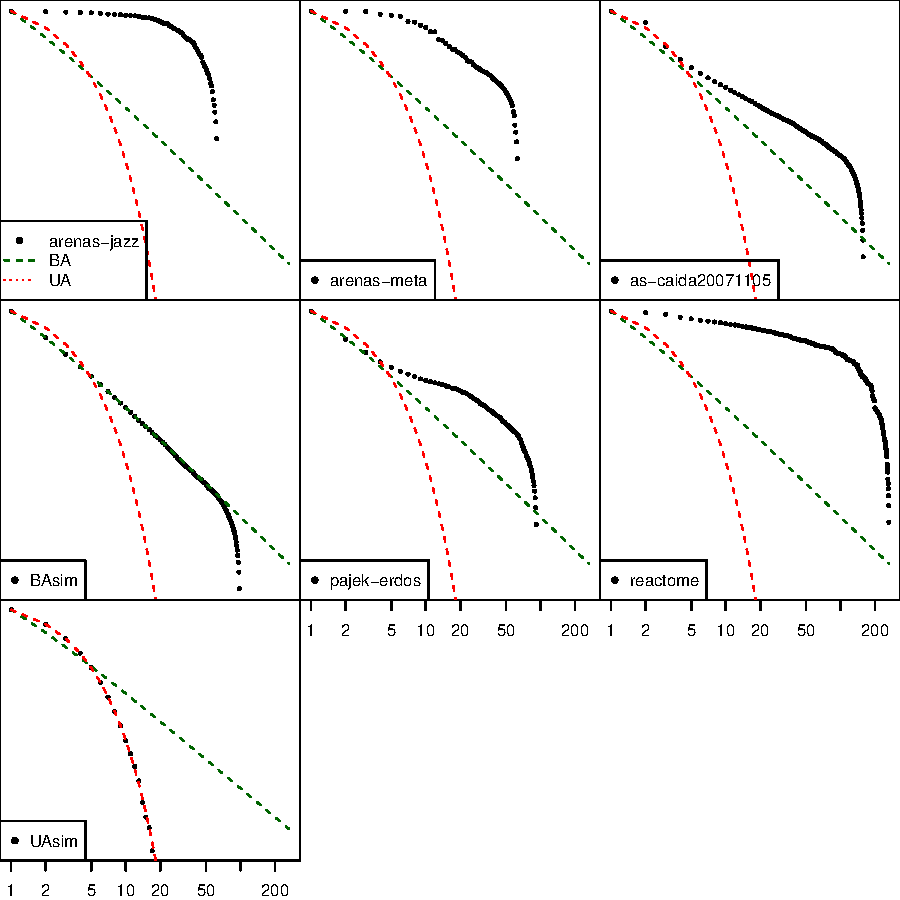
\includegraphics[width=0.9\textwidth,height=\textheight]{doc_files/figure-pdf/fig-survs-1.pdf}

}

\caption{\label{fig-survs}Survival function of the degrees.}

\end{figure}

The shapes of the curves in Figure~\ref{fig-survs} are all fairly
different but, they all seem to start with what looks like one power law
and then begins to deviate after a certain point indicating the while
the bulk of the data follows the one power law the right tail does not
necessarily exhibit the same behaviour. Seeing this and with the aim of
investigating the tail-heaviness of networks degree distributions,
fitting a model that uses a power law for the bulk of the data and the
IGP distribution (Definition~\ref{def-igp}) for the right tail above a
certain threshold should allow for estimation of the tail-index.

\hypertarget{power-law-igp-mixture-model-pl-igp}{%
\subsection{Power Law IGP Mixture Model
(PL-IGP)}\label{power-law-igp-mixture-model-pl-igp}}

A traditional way of modelling continuous extreme values often involves
using the GP distribution (Definition~\ref{def-gp}) to model the
conditional distribution of the largest values however here the data is
discrete and so instead the IGP will be used as an alternative. For the
bulk of the data a truncated power law distribution will be used which
is defined in Definition~\ref{def-tpl} below, and for the right tail the
IGP will be used.

\begin{definition}[Truncated Power
Law]\protect\hypertarget{def-tpl}{}\label{def-tpl}

The truncated power law distribution has two parameters
\(\alpha \in \mathbb R\),\(v \in \mathbb Z^+\) and has support of
\((1,v)\). The pdf of this distribution is: \[
f(x) = \begin{cases}
\frac{x^{-(\alpha+1)}}{\sum_{i=1}^v i^{-(\alpha+1)}}&,x=1,2,\ldots,v\\
0&,\text{otherwise}
\end{cases}
\]

\end{definition}

\hypertarget{network-generative-models}{%
\section{Network Generative Models}\label{network-generative-models}}

The way in which vertices and edges are added and removed from networks
over time is of great interest as it can lead to inferences about the
underlying mechanics of a complex system and allow for theorising what
may happen to the network in the future. To that end, finding a model
that is both simple enough and leads to properties that match real world
networks is of utmost importance. Next, the degree distribution of
various network models are analysed starting fairly simple and
gradualling getting more complex.

\begin{definition}[Uniform attachment
model]\protect\hypertarget{def-uniform}{}\label{def-uniform}

Consider an initial graph \(G_0\) with vertex set
\(V_0=\{1,2,\ldots,m_0\}\) and edge set \(E_0=\emptyset\). Starting at
\(t=1\) repeat the steps below:

\begin{enumerate}
\def\labelenumi{\arabic{enumi}.}
\tightlist
\item
  Add a vertex to the network, \(V_t=V_{t-1}\cup\{m_0+t\}\)
\item
  Add \(m\le m_0\) edges to the network connecting the new vertex to
  those in already in the network. With the existing vertices to be
  chosen uniformly at random from \(V_{t-1}\) with replacement.
\end{enumerate}

\end{definition}

\newpage{}

\hypertarget{references}{%
\chapter*{References}\label{references}}
\addcontentsline{toc}{chapter}{References}

\hypertarget{refs}{}
\begin{CSLReferences}{1}{0}
\leavevmode\vadjust pre{\hypertarget{ref-Rohrbeck_2018}{}}%
Rohrbeck, Christian, Emma F. Eastoe, Arnoldo Frigessi, and Jonathan A.
Tawn. 2018. {``{Extreme value modelling of water-related insurance
claims}.''} \emph{The Annals of Applied Statistics} 12 (1): 246--82.
\url{https://doi.org/10.1214/17-AOAS1081}.

\leavevmode\vadjust pre{\hypertarget{ref-shimura12}{}}%
Shimura, Takaaki. 2012. {``Discretization of Distributions in the
Maximum Domain of Attraction.''} \emph{Extremes} 15 (September): 1--19.
\url{https://doi.org/10.1007/s10687-011-0137-7}.

\end{CSLReferences}



\end{document}
